% Draft: compile with the official IEEEtran conference class, A4 paper.
% Replace both author identifiers before submission. No abstract per Ed #156.
% Page count must be checked after compilation; do not shrink IEEE fonts/margins.
\RequirePackage[T1]{fontenc}
\documentclass[conference,a4paper]{IEEEtran}
\usepackage{amsmath,amssymb}
\usepackage{graphicx}
\usepackage{url}
\usepackage[hidelinks]{hyperref}
\title{House Price Prediction with Frozen Visual Features and Kernel Fusion}
\author{\IEEEauthorblockN{Shifeng Chen \qquad Haoxuan Ying}
\IEEEauthorblockA{1686631 \qquad 1255329\\
COMP90086 Computer Vision, The University of Melbourne}}
\begin{document}
\maketitle
\raggedbottom

\section{Introduction}
Estimating a house's sale price involves size, condition, location and market conditions. Exterior photographs reveal some of this information: computer vision can describe architectural form, surface appearance, landscaping and surrounding scenes. However, a single view provides incomplete coverage and does not directly reveal floor area, an exact address or transaction conditions. We therefore investigate how to extract more informative visual features from house photographs to predict sale prices more accurately.

Visual representations offer several approaches. Handcrafted descriptors summarize local gradients and textures, while networks such as AlexNet~\cite{alexnet} learn hierarchical features. Large-scale pretraining further enables transfer across tasks: CLIP~\cite{clip}, SigLIP2~\cite{siglip2} and Perception Encoder~\cite{pe} motivate freezing the visual encoder and learning price regression separately.

Our study follows three stages. SIFT with a visual vocabulary first tests whether local appearance predicts price. An AlexNet-style regressor then undergoes controlled training, augmentation and architecture experiments. Its remaining error motivates frozen pretrained features, for which we investigate image coverage, feature transformation and regression before combining complementary branches.

The selected three-encoder fusion achieves validation MSE 52,201.21 and MAE 159.58, with public Kaggle MSE 47,291.35 after full-data refitting. Our analysis relates these gains to representation and kernel design, while identifying persistent high-price underestimation and uneven benefits across price groups.

\section{Methods}
\subsection{Data, Metrics and Evaluation Protocol}
The dataset contains 8,000 labelled training images and 3,000 unlabelled test images from Southern California real-estate listings. Prices are measured in thousand USD. We fit the models using the supplied images and prices, with general-purpose pretrained image encoders providing transferable visual features.

We split the data into 6,399 training and 1,601 validation images with seed 2026, keeping identified duplicate or related-image groups together. For $N$ evaluated images with true prices $y_i$ and predictions $\hat y_i$, we report
\begin{equation}
\mathrm{MSE}=\frac{1}{N}\sum_{i=1}^{N}(\hat y_i-y_i)^2,\qquad
\mathrm{MAE}=\frac{1}{N}\sum_{i=1}^{N}|\hat y_i-y_i|.
\end{equation}
MSE, the primary metric, emphasizes large errors; MAE measures average absolute error. Their units are (thousand USD)$^2$ and thousand USD, respectively. Signed residuals $\hat y_i-y_i$ describe bias.

Stochastic models are screened with seed 2026; promising candidates are repeated with seeds 2027 and 2028. Adoption requires lower mean MSE and at least two seed-matched wins; we report means and sample standard deviations. Frozen-feature regressors use grouped three-fold training out-of-fold (OOF) selection, fitting codebooks, scalers, PCA and supervised transforms within each fold.

\subsection{Baselines and Controlled CNN Development}
We first predict the training mean as a non-visual reference. To determine whether local appearance adds information, we extract grayscale SIFT descriptors~\cite{sift1999,sift} and build a 256-word visual vocabulary~\cite{bovw}. Histograms undergo L1--square-root--L2 normalization and standardization before Ridge regression~\cite{ridge} ($\alpha=10$). Although this captures local gradient structure, pooling into a histogram discards spatial arrangement. We therefore also examine a CNN that learns feature composition directly from images.

Our AlexNet-style regressor~\cite{alexnet} has five convolutional layers and a 9216--4096--4096--1 head, initialized from scratch. After preprocessing comparisons, the selected input is a direct $224\times224$ resize, RGB normalization with mean and SD 0.5, and no filtering. The retained configuration uses AdamW~\cite{adamw} ($10^{-4}$ learning rate and weight decay), dropout~\cite{dropout2012,dropout} 0.5, and effective batch 32 through microbatch 4 and eight-step accumulation. Training uses prices divided by 1,000; predictions are restored to dataset units. Runs last at most 60 epochs, with a minimum of 40 and patience 15 under a 0.1\% improvement stopping rule; the checkpoint with strictly lowest validation MSE is retained.

We first compare learning rates, optimizers including Adam~\cite{adam}, cosine decay~\cite{sgdr} without restarts, effective batch size, regularization and initialization~\cite{xavier,heinit}, then test augmentation. Geometric and degradation transforms are evaluated separately; horizontal flip uses probability 0.5. Architecture experiments test stacked $3\times3$ convolutions~\cite{vgg} replacing the second $5\times5$ layer, an Inception-style multi-scale block~\cite{inception}, and a projected residual connection~\cite{resnet}. To reduce the large fully connected head, we project the $6\times6$ convolutional grid to 128 channels, add positional information and normalization, and average the 36 tokens before linear regression. We then test a one-layer Transformer~\cite{transformer} with dimension 128, four heads and a 512-dimensional feed-forward layer. Each change is evaluated against its corresponding control.

In a separate seed-2026 screen, brightness and contrast are each multiplied by a factor sampled uniformly from $[0.9,1.1]$ on every training image before resizing and normalization. Both are compared with a freshly trained unaugmented AlexNet using the same initialization, split and training settings.

\subsection{Frozen Representations, Views and Regression}
To extend the scratch models, we decouple visual representation from price regression. Frozen CLIP ViT-B/32 features with standardized Ridge regression establish the transfer-learning reference; the final branches use SigLIP2 So400m NaFlex, PE-Core-L/14 and PE-Core-G/14. NaFlex preserves native aspect ratio with 576 patches and produces 1,152-dimensional features. Because a single crop can remove useful context, PE-L combines three 1,024-dimensional views: the official input, a 336-pixel gray-padded whole frame, and a central crop spanning 60\% of image width and height. PE-G combines its official 448-pixel view with a gray-padded whole frame. Features are individually unit-normalized, concatenated and normalized again, yielding 3,072 PE-L and 2,560 PE-G dimensions.

We use RBF kernel ridge regression~\cite{krr} to model nonlinear relationships in the frozen feature space, with regularization controlling the fitted coefficients. For unit features $x$,
\begin{equation}
 K_{ij}=\exp(-\gamma\|x_i-x_j\|^2),\quad
 c=(K+\alpha I)^{-1}(y-\bar y\mathbf{1}),
\end{equation}
with prediction $\bar y+k(x)^Tc$ and non-negative clipping. Ordinary kernel searches use $\gamma\in\{1,4,16\}$ and $\alpha\in\{0.01,0.1,1,10\}$ on training folds. NaFlex selects $\gamma=1$, $\alpha=0.1$.

However, generic visual similarity may emphasize variation unrelated to price. PE-L therefore uses fold-fitted PLS~\cite{pls1966,pls} to learn price-related directions. Sixteen components are fitted; the selected head uses the first four standardized scores $s$ and the product kernel
\begin{equation}
 k(x,x')=\exp\left(-\|x-x'\|^2-0.1\frac{\|s-s'\|^2}{4}\right),
\end{equation}
with $\alpha=1$. The PLS scores introduce price-related directions into the similarity measure while keeping the image encoder frozen.

In contrast to supervised PLS, PCA~\cite{pca} compresses features along their principal variation directions without using prices. For PE-G, we test 64, 256 and 1,024 dimensions with whitening powers 0 and 0.5, followed by unit normalization. Since this changes distances, we also recalibrate the original $\gamma=4$:
\begin{equation}
 \gamma'=4\frac{\operatorname{median}\|x_i-x_j\|^2}
 {\operatorname{median}\|z_i-z_j\|^2},
\end{equation}
using 8,192 fixed non-self pairs drawn only from fitting-fold images. Here $z$ is the transformed unit vector. The selected transform is non-whitened PCA256 with $\alpha=1$.

\subsection{Fusion and Final Refit}
Following stacked regression~\cite{stacking}, we combine branch predictions using non-negative weights, additionally constrained to sum to one. Weights are fitted to training OOF predictions and evaluated by meta cross-fitting: each fold is predicted using weights fitted on the remaining folds. A new branch is retained when meta-CV MSE improves by at least 1\%, at least two of three folds improve, and validation MSE also decreases.

The final weights are NaFlex 0.108065, PE-L PLS 0.080806 and PE-G PCA 0.811129. For the Kaggle submission, we retain the selected hyperparameters and weights and refit the transforms and regression heads on all 8,000 labelled images, recomputing PCA and bandwidth statistics from this training set. The fitted model then predicts the 3,000 test prices.

\section{Results}
% Native two-column IEEE table; no additional LaTeX package required.
\begin{table*}[t]
\centering
\caption{Representative configurations evaluated on the fixed validation split.}
\label{tab:representative-results}
\small
\setlength{\tabcolsep}{4pt}
\renewcommand{\arraystretch}{1.0}
\begin{tabular*}{\textwidth}{@{\extracolsep{\fill}}lcr@{\,}c@{\,}rr@{}}
\hline
Method & Seeds & \multicolumn{3}{c}{Validation MSE} & Validation MAE \\
\hline
AlexNet (no augmentation) & 3 & 127,774 & $\pm$ & 486 & 264.52 \\
AlexNet (Adam, lr=0.001) & 3 & 128,284 & $\pm$ & 1,106 & 264.80 \\
AlexNet + horizontal flip & 3 & 126,810 & $\pm$ & 1,902 & 268.02 \\
Flip AlexNet + small-kernel stack & 1 & 127,320 &  &  & 262.19 \\
Flip AlexNet + mean-pooling head & 3 & 122,334 & $\pm$ & 1,589 & 261.48 \\
Mean-pooling head + Transformer & 1 & 124,389 &  &  & 259.55 \\
Frozen CLIP B32 + Ridge & -- & 91,821 &  &  & 223.27 \\
Frozen PE-G, two views + PCA/KRR & -- & 52,806 &  &  & 160.67 \\
\textbf{Selected three-encoder fusion} & \textbf{--} & \textbf{52,201} & \textbf{} & \textbf{} & \textbf{159.58} \\
\hline
\end{tabular*}
\par\smallskip
\begin{minipage}{0.96\textwidth}
\scriptsize
Validation $n=1{,}601$. MSE: (thousand USD)$^2$; MAE: thousand USD.
Three-seed results report MSE mean $\pm$ sample SD and MAE mean.
Single-seed results use seed 2026; -- indicates frozen-feature evaluation.
\end{minipage}
\end{table*}

\begin{figure*}[t]
\centering
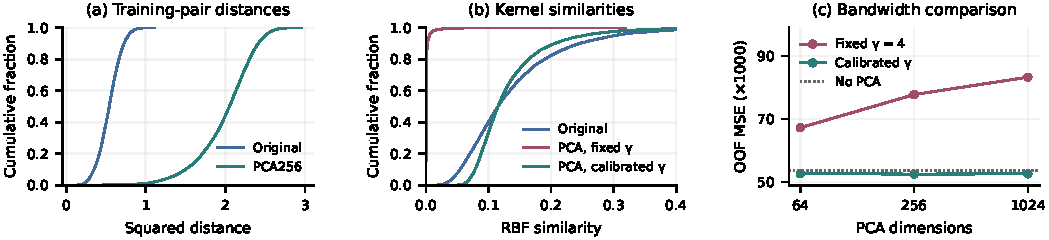
\includegraphics[width=\textwidth]{figures/report_pca_distance_bandwidth_oof.pdf}
\caption{PE-G geometry and regression. (a,b) Empirical CDFs of distances and kernel similarities for 8,192 training pairs; (c) grouped three-fold OOF MSE for non-whitened PCA. Transforms and bandwidths are fitted within each fold. Panel (b) shows the similarity range 0--0.4.}
\label{fig:pca}
\end{figure*}
\begin{figure*}[t]
\centering
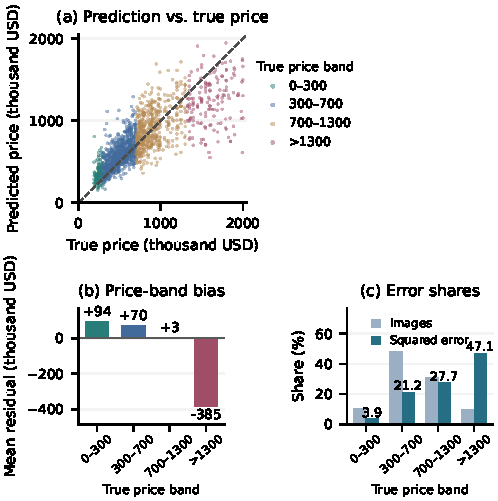
\includegraphics[width=\textwidth]{figures/report_prediction_scatter_price_band_errors.pdf}
\caption{Selected fusion on 1,601 validation images. (a) Predicted versus true price; the dashed line is perfect prediction and colors follow the price bands in (b). (b) Mean residual $\hat y-y$. (c) Image and squared-error shares. Bands are $(0,300]$, $(300,700]$, $(700,1300]$ and above 1,300 thousand USD.}
\label{fig:errors}
\end{figure*}
\begin{figure*}[t]
\centering
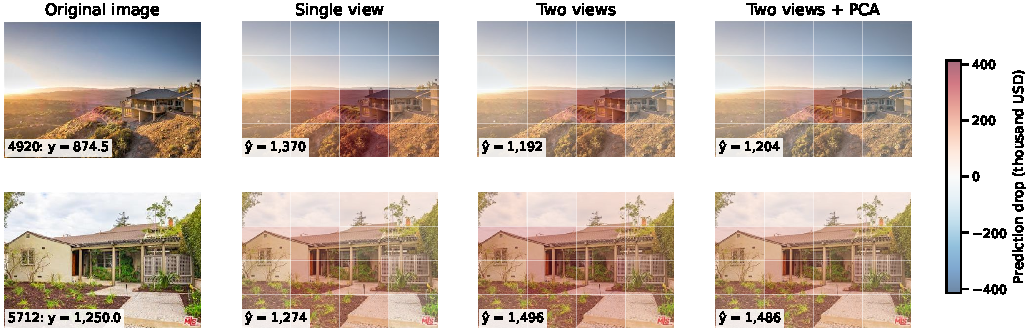
\includegraphics[width=\textwidth]{figures/report_pe_g_occlusion_model_comparison.pdf}
\caption{Regional sensitivity of three PE-G regression pipelines under $4\times4$ blur replacement. Rows show the largest improvement (4920) and worsening (5712) after adding the whole frame among 1,543 landscape validation images. Red indicates that replacement lowers the prediction; blue indicates an increase. All maps share one scale; labels give true ($y$) and unperturbed predicted ($\hat y$) prices in thousand USD.}
\label{fig:occlusion}
\end{figure*}

\subsection{From Baselines to Frozen Visual Features}
The mean predictor obtains MSE 151,839.69; SIFT--BoVW--Ridge reduces this to $145,336.73\pm1,091.58$ across three seeds. Local appearance therefore contains a measurable, limited price signal. The original padded-input AlexNet obtains mean MSE 128,415.68. Table~\ref{tab:representative-results} starts from its direct-resize successor, 127,774.42, which is the matched no-augmentation reference for subsequent training experiments.

Optimization alone provides little improvement. Although Adam at learning rate 0.001 improves seed 2026, it loses the other two paired comparisons and increases mean MSE by 509.89. Likewise, cosine scheduling, alternative batch sizes and lower dropout fail the three-seed adoption criterion, so the original training settings are retained.

With these settings fixed, horizontal flip reduces mean MSE by 964.41 with two paired wins, although MAE rises from 264.52 to 268.02. A clearer gain comes from the mean-pooling head: it improves all three seeds and reduces MSE by 4,475.78 relative to flip AlexNet. In contrast, small-kernel, multi-scale and residual screens fail to improve their controls, while a Transformer increases MSE by 3,615.11 over the small head in the single-seed screen. We therefore retain the compact head.

The separate photometric screen gives MSE 131,389.94 and MAE 282.64 for its fresh control. Brightness leaves MSE almost unchanged at 131,433.91 while reducing MAE to 274.50. Contrast lowers MSE to 128,860.53 (1.93\%) and MAE to 269.01, but increases MSE for prices above 1,300 by 17.14\%; brightness increases this tail metric by 3.86\%. Contrast's gains in the two lower price bands outweigh deterioration in both upper bands. It is therefore a candidate for further paired-seed evaluation, rather than a confirmed replacement for the retained augmentation.

The scratch experiments thus yield modest improvements. Frozen CLIP with Ridge reduces validation MSE to 91,820.73, motivating richer pretrained representations and more effective readouts.

\subsection{Image Coverage and Kernel Geometry}


Adding the whole frame to PE-G reduces single-branch validation MSE from 55,097.49 to 53,252.81 and OOF MSE from 55,679.73 to 53,646.46, supporting the value of peripheral context alongside the official view.

PCA256 worsens OOF MSE to 77,771.43 with fixed $\gamma=4$, but calibration reduces it to 52,531.27. The development-training median squared distance rises from 0.5402 to 2.0515, giving calibrated $\gamma=1.05323$ (Fig.~\ref{fig:pca}). Validation MSE reaches 52,805.77 and MAE 160.67. Thus, feature transformation needs to be evaluated jointly with bandwidth.

Adding this branch to the preceding fusion lowers meta-CV MSE from 53,052.57 to 52,210.22, with all three folds improving, and validation MSE from 52,524.78 to 52,201.21. The corresponding public Kaggle MSE improves from 47,837.69 to 47,291.35.

\subsection{Fusion Complementarity}
With branch predictions fixed, we refit weights after each removal. Without PE-G PCA, validation MSE rises to 57,372.90; without NaFlex, it reaches 52,597.50. Equal weights give 53,847.68, supporting learned fusion. Removing PE-L slightly improves validation MSE to 52,194.81 but raises meta-CV MSE from 52,210.22 to 52,244.24. The training-side criterion therefore retains the full fusion, dominated by PE-G.

\subsection{Error Analysis and Regional Sensitivity}


The final model has RMSE 228.48, median absolute error 113.41 and mean residual $+6.51$. This small overall bias masks opposing price-dependent errors (Fig.~\ref{fig:errors}): mean residual is $+93.72$ below or equal to 300, but $-385.16$ above 1,300. The 159 highest-price images have MAE 410.90 and account for 47.13\% of total squared error. Errors are concentrated in a small subset: the 161 largest absolute errors account for 63.30\% of squared error.

The last fusion improvement is heterogeneous. Lowest- and highest-price bands contribute $-224.23$ and $-882.25$ to the overall MSE change, while the middle bands contribute $+185.43$ and $+597.48$. Their sum is $-323.57$. Better aggregate MSE therefore does not imply that all price groups improve.

Extreme-error cases illustrate the difficulty of estimating value from appearance. Image 5352 shows a terrace and distant sea view, yet its prediction of 1,679.82 substantially exceeds the true price of 949.0. Conversely, image 2138 shows a wood-clad house priced at 1,995.0 but predicted at 605.27. These examples suggest that visible appearance and context can be ambiguous indicators of value.

Using regional occlusion~\cite{occlusion}, we examine images 4920 and 5712, the largest improvement and worsening after adding the whole frame among 1,543 landscape validation images. Each $4\times4$ region is replaced with gray pixels or a radius-8 Gaussian-blurred version. Figure~\ref{fig:occlusion} compares the blur responses of the single-view, two-view and PCA PE-G models. Their largest responses overlap house regions. However, for the two-view model on 5712, the gray/blur correlation is only 0.267. The maps therefore describe sensitivity to a particular perturbation, rather than reliably identifying specific price-related attributes.

\section{Discussion}
The three routes reveal different requirements for visual valuation. Handcrafted SIFT features explicitly represent local appearance, but visual-word pooling discards spatial relationships, potentially limiting discrimination between properties with different building and environmental layouts. This highlights the importance of organizing image evidence.

The scratch-CNN route makes this organization learnable, but requires learning features and price relationships from limited supervision. The compact head suggests that matching capacity to available labels can be more useful than architectural complexity. Greater expressive power therefore does not automatically produce more informative price features.

Frozen pretrained encoders supply knowledge learned beyond the price-labelled dataset, allowing task learning to focus on regression. Adaptation remains essential: views determine which evidence survives preprocessing, while transforms and kernel geometry connect visual similarity to price. Caching enables reuse on limited hardware, although dense kernels constrain scalability; fusion exploits complementary representations with unequal contributions.

Together, accurate prediction requires informative representations, adequate coverage and a mapping aligned with valuation. Appearance provides partial evidence of value; unobserved location, floor area and transaction conditions may explain remaining ambiguity. Future work should connect spatial and contextual features more directly to price differences. Multiple component changes and reused development data also warrant independent grouped evaluation.

\clearpage
\IEEEtriggeratref{14}
\begin{thebibliography}{99}
\bibitem{alexnet} A. Krizhevsky, I. Sutskever, and G. E. Hinton, ``\href{https://papers.nips.cc/paper_files/paper/2012/hash/c399862d3b9d6b76c8436e924a68c45b-Abstract.html}{ImageNet classification with deep convolutional neural networks},'' \emph{Advances in Neural Information Processing Systems, vol. 25}, 2012.
\bibitem{clip} A. Radford et al., ``\href{https://proceedings.mlr.press/v139/radford21a.html}{Learning transferable visual models from natural language supervision},'' \emph{Proc. ICML}, 2021, pp. 8748--8763.
\bibitem{siglip2} M. Tschannen et al., ``\href{https://arxiv.org/abs/2502.14786}{SigLIP 2: Multilingual vision-language encoders with improved semantic understanding, localization, and dense features},'' \emph{arXiv:2502.14786}, 2025.
\bibitem{pe} D. Bolya et al., ``\href{https://arxiv.org/abs/2504.13181}{Perception Encoder: The best visual embeddings are not at the output of the network},'' \emph{arXiv:2504.13181}, 2025.
\bibitem{sift1999} D. G. Lowe, ``\href{https://www.cs.ubc.ca/~lowe/papers/iccv99.pdf}{Object recognition from local scale-invariant features},'' \emph{Proc. ICCV}, 1999, pp. 1150--1157.
\bibitem{sift} D. G. Lowe, ``\href{https://www.cs.ubc.ca/~lowe/papers/ijcv04.pdf}{Distinctive image features from scale-invariant keypoints},'' \emph{International Journal of Computer Vision, vol. 60}, 2004, pp. 91--110.
\bibitem{bovw} J. Sivic and A. Zisserman, ``\href{https://www.robots.ox.ac.uk/~vgg/publications/2003/Sivic03/}{Video Google: A text retrieval approach to object matching in videos},'' \emph{Proc. ICCV}, 2003, pp. 1470--1477.
\bibitem{ridge} A. E. Hoerl and R. W. Kennard, ``\href{https://doi.org/10.1080/00401706.1970.10488634}{Ridge regression: Biased estimation for nonorthogonal problems},'' \emph{Technometrics, vol. 12}, 1970, pp. 55--67.
\bibitem{adamw} I. Loshchilov and F. Hutter, ``\href{https://arxiv.org/abs/1711.05101}{Decoupled weight decay regularization},'' \emph{Proc. ICLR}, 2019.
\bibitem{dropout2012} G. E. Hinton et al., ``\href{https://arxiv.org/abs/1207.0580}{Improving neural networks by preventing co-adaptation of feature detectors},'' \emph{arXiv:1207.0580}, 2012.
\bibitem{dropout} N. Srivastava et al., ``\href{https://jmlr.org/papers/v15/srivastava14a.html}{Dropout: A simple way to prevent neural networks from overfitting},'' \emph{Journal of Machine Learning Research, vol. 15}, 2014, pp. 1929--1958.
\bibitem{adam} D. P. Kingma and J. Ba, ``\href{https://arxiv.org/abs/1412.6980}{Adam: A method for stochastic optimization},'' \emph{Proc. ICLR}, 2015.
\bibitem{sgdr} I. Loshchilov and F. Hutter, ``\href{https://arxiv.org/abs/1608.03983}{SGDR: Stochastic gradient descent with warm restarts},'' \emph{Proc. ICLR}, 2017.
\bibitem{xavier} X. Glorot and Y. Bengio, ``\href{https://proceedings.mlr.press/v9/glorot10a.html}{Understanding the difficulty of training deep feedforward neural networks},'' \emph{Proc. AISTATS}, 2010, pp. 249--256.
\bibitem{heinit} K. He et al., ``\href{https://openaccess.thecvf.com/content_iccv_2015/html/He_Delving_Deep_into_ICCV_2015_paper.html}{Delving deep into rectifiers: Surpassing human-level performance on ImageNet classification},'' \emph{Proc. ICCV}, 2015, pp. 1026--1034.
\bibitem{vgg} K. Simonyan and A. Zisserman, ``\href{https://arxiv.org/abs/1409.1556}{Very deep convolutional networks for large-scale image recognition},'' \emph{Proc. ICLR}, 2015.
\bibitem{inception} C. Szegedy et al., ``\href{https://openaccess.thecvf.com/content_cvpr_2015/html/Szegedy_Going_Deeper_With_2015_CVPR_paper.html}{Going deeper with convolutions},'' \emph{Proc. CVPR}, 2015, pp. 1--9.
\bibitem{resnet} K. He et al., ``\href{https://openaccess.thecvf.com/content_cvpr_2016/html/He_Deep_Residual_Learning_2016_CVPR_paper.html}{Deep residual learning for image recognition},'' \emph{Proc. CVPR}, 2016, pp. 770--778.
\bibitem{transformer} A. Vaswani et al., ``\href{https://papers.nips.cc/paper_files/paper/2017/hash/3f5ee243547dee91fbd053c1c4a845aa-Abstract.html}{Attention is all you need},'' \emph{Advances in Neural Information Processing Systems, vol. 30}, 2017.
\bibitem{krr} C. Saunders, A. Gammerman, and V. Vovk, ``\href{https://eprints.soton.ac.uk/258942/}{Ridge regression learning algorithm in dual variables},'' \emph{Proc. ICML}, 1998, pp. 515--521.
\bibitem{pls1966} H. Wold, ``Estimation of principal components and related models by iterative least squares,'' \emph{Multivariate Analysis, P. R. Krishnaiah, Ed. Academic Press}, 1966, pp. 391--420.
\bibitem{pls} S. Wold, A. Ruhe, H. Wold, and W. J. Dunn III, ``\href{https://doi.org/10.1137/0905052}{The collinearity problem in linear regression. The partial least squares (PLS) approach to generalized inverses},'' \emph{SIAM Journal on Scientific and Statistical Computing, vol. 5}, 1984, pp. 735--743.
\bibitem{pca} K. Pearson, ``\href{https://doi.org/10.1080/14786440109462720}{On lines and planes of closest fit to systems of points in space},'' \emph{Philosophical Magazine, vol. 2}, 1901, pp. 559--572.
\bibitem{stacking} L. Breiman, ``\href{https://doi.org/10.1007/BF00117832}{Stacked regressions},'' \emph{Machine Learning, vol. 24}, 1996, pp. 49--64.
\bibitem{occlusion} M. D. Zeiler and R. Fergus, ``\href{https://arxiv.org/abs/1311.2901}{Visualizing and understanding convolutional networks},'' \emph{Proc. ECCV}, 2014, pp. 818--833.
\end{thebibliography}
\end{document}
